\chapter{Groundwork, Libraries and tools}

\section{Existing work}

As often happens in this field, most of the results presented stem from the work that other talented people have done before.
This is particularly true since the project aims to refactor an existing codebase, understand the algorithms used and extend the software with some commodities and functionalities.
While most of the project's inner workings have not changed, if not for some slight modifications for clarity or performance, the integration with the build system and the dependencies has been altered significantly.
Furthermore, since the repository started as a fork of \dreal \cite{repo:dreal}, many of the original files had been kept even when unused, needlessly cluttering the filesystem.
Another important aspect is the addition of a benchmark framework and the \texttt{python} bindings, which facilitates use for the end user.

\section{External libraries}

\subsection*{spdlog and argparse}

spdlog is a fast, header-only/compiled logging library \cite{repo:spdlog}.
It uses the \texttt{fmt} formatting library to ease the creation of the log messages and supports many log targets and levels.

argparse is a \texttt{c++17} header-only library for parsing command line arguments \cite{repo:argparse}.
It provides an interface reminiscent of the \texttt{python} library with the same name and is very easy to use.

\subsection*{gmp}

gmp is a free library for arbitrary precision arithmetic, operating on signed integers, rational numbers, and floating-point numbers.
There is a significant focus on being as fast as possible for small and huge operands.
Such speed is achieved using fullwords as the basic arithmetic type and fast algorithms, with highly optimised assembly \cite{man:gmp}.
It is used in many applications dealing with any kind of mathematical computation with large numbers or very high precision.

There are several categories of functions provided by the library.
For this project, the most relevant ones are the \textit{high-level rational arithmetic} function using the \texttt{mpq} type.
The \texttt{mpz} functions can be used, too, by applying them to the numerator and denominator separately.

\subsection*{Soplex}

SoPlex is an open-source optimisation solver for \gls{lp} problems based on an advanced implementation of the primal and dual revised simplex algorithm.
It provides special support for the exact solution of LPs with rational input data.
It can be easily embedded into other programs via a C++ class library.

SoPlex has been used in numerous research and industry projects and is the standard LP solver linked to the mixed-integer nonlinear programming and constraint integer programming solver SCIP \cite{man:soplex}.

\subsection*{Qsopt\_ex}

Qsopt\_ex was developed as a specialisation of the Qsopt library to obtain exact solutions to \gls{lp} problems \footnote{\url{https://www.math.uwaterloo.ca/~bico/qsopt/ex/}}.
The original library was then forked and extended two times.
Under the Debian Med group, the first fork updated the software and the build system to be more friendly \footnote{\url{https://salsa.debian.org/med-team/qsopt-ex}}.
Finally, Martin Sidaway adapted the software to support solving the delta-weakening of the problem \cite{repo:qsopt-ex}.
The last one is the version used in \dlinear.

\section{Build tools}

When dealing with large projects written in \texttt{c++}, it is common to use a build system to automate the compilation process, manage dependencies and run tests.
Some of the most popular build systems are \textit{CMake} \footnote{\url{https://cmake.org/}}, \textit{msbuild} \footnote{\url{https://learn.microsoft.com/visualstudio/msbuild/msbuild}} and \textit{Makefiles} (\autoref{fig:cpp_build_systems}).
Still, less conventional tools find their niche, such as \textit{Bazel} \footnote{\url{https://bazel.build/}}.

\begin{figure}[h]
    \centering
    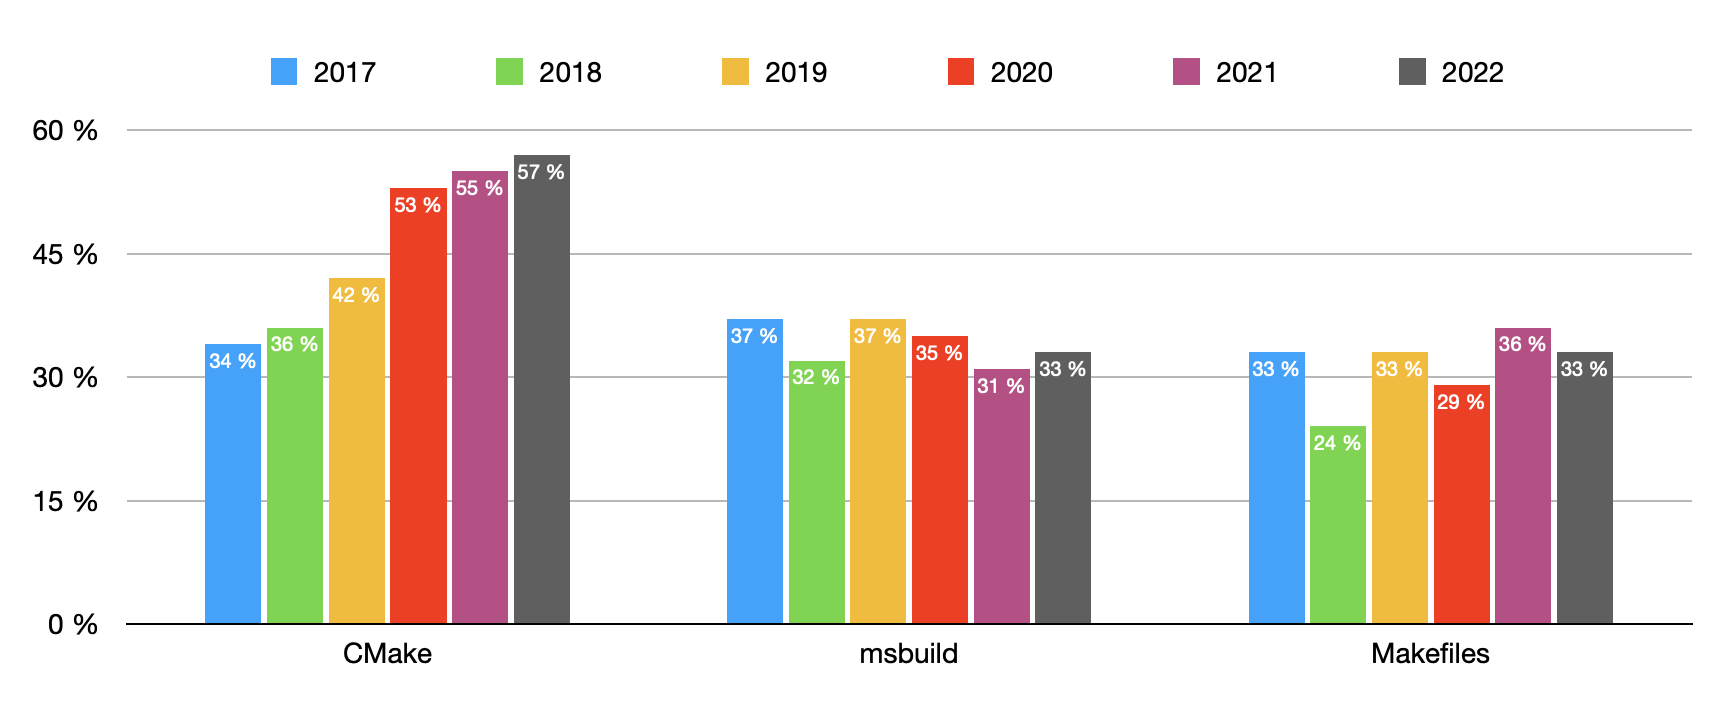
\includegraphics[width=0.65\textwidth]{cpp_build_systems}
    \caption{Comparison of the most popular build systems for \texttt{c++} projects \cite{art:cpp-build-system}}\label{fig:cpp_build_systems}
\end{figure}

Following the footsteps of the original authors, the choice fell on \textit{Bazel} \cite{repo:bazel}.
It is an open-source build system developed and maintained by Google.
It supports multiple languages and platforms and is designed to scale well with large projects, thanks to its incremental builds and caching mechanisms.

\bazel's primary goals are reproducibility and correctness, achieved by using a declarative language to define the build process and using a sandboxed environment to run the build actions.
This ensures that the build process is deterministic and that the build actions do not have side effects: all inputs and outputs must be explicitly declared for each rule.

It also features a domain-specific language \texttt{starlark} \cite{repo:starlark}, used to customize the build process even further, adding support for personalized rules and macros.
The syntax is intentionally very similar to the familiar \texttt{python}, although some more advanced language features are not included.
Custom scripts can also be shared among users, allowing the creation of packages of specialized rules for many use cases.

\subsection*{Configuration}

The \textit{Bazel} \textit{workspace} is the top-level directory.
It contains all the source files of the project, as well as scripts and configuration files.
It is defined by the presence of a \texttt{WORKSPACE.bazel} file, which specifies the project's name and is a common place to define the external dependencies.

\lstinputlisting[language=bazel,frame=single,showstringspaces=false,caption={Example of a \texttt{WORKSPACE.bazel} file},captionpos=b,label={code:workspace}]{code/example.WORKSPACE.bazel}

The project can be split into multiple \textit{packages}, each defined by a \texttt{BUILD.bazel} file.
This greatly simplifies the build process, as it is possible to build a complete dependency graph and rebuild only the smallest subset of the project when it has been modified, using the cache for the rest.

\lstinputlisting[language=bazel,frame=single,showstringspaces=false,caption={Example of a \texttt{Build.bazel} file},captionpos=b,label={code:build}]{code/example.BUILD.bazel}

\subsection*{Dependencies}

\textit{Bazel} provides the means to manage internal and external dependencies.
The external dependencies are downloaded and built from source to ensure isolation and reproducibility.
Most libraries do not provide a \texttt{BUILD.bazel} file since they employ a different build system.
In those cases, it is necessary to write one manually, specifying the source files, the dependencies and the compilation flags.
To aid in the compilation, there exist several rules that ensure interoperability with the most common tools, such as \textit{CMake}, \textit{configure-make}, \textit{GNU Make}, \textit{boost}, \textit{ninja} and \textit{Meson} \cite{repo:rules-foreign-cc}.

\lstinputlisting[language=bazel,frame=single,showstringspaces=false,caption={Inclusion of the foreign_rules_cc in the WORKSPACE.bazel file},captionpos=b,label={code:foreign_cc.WORKSPACE.bazel}]{code/foreign\_cc.WORKSPACE.bazel}

The two solvers that \dlinear uses need to be included as the project's dependencies.
In the original setup, it was necessary to download the source code and compile it manually, which was a tedious process.
This step was automated by creating an ad hoc \texttt{BUILD.bazel} file for each of them, which is used when building the project.
It also allows us to specify whether to use them as static libraries for the main executable or as dynamic libraries for the \texttt{python} bindings.

\lstinputlisting[language=bazel,frame=single,showstringspaces=false,caption={Simplified \texttt{BUILD.bazel} file for the SoPlex library},captionpos=b,label={code:soplex.BUILD.bazel}]{code/soplex.BUILD.bazel}

\bazel includes a utility that shows the project's dependency graph, which gives a good overview of the couplings between the different components.
The result is \autoref{fig:dlinear-deps}.

\begin{figure}[h]
    \centering
    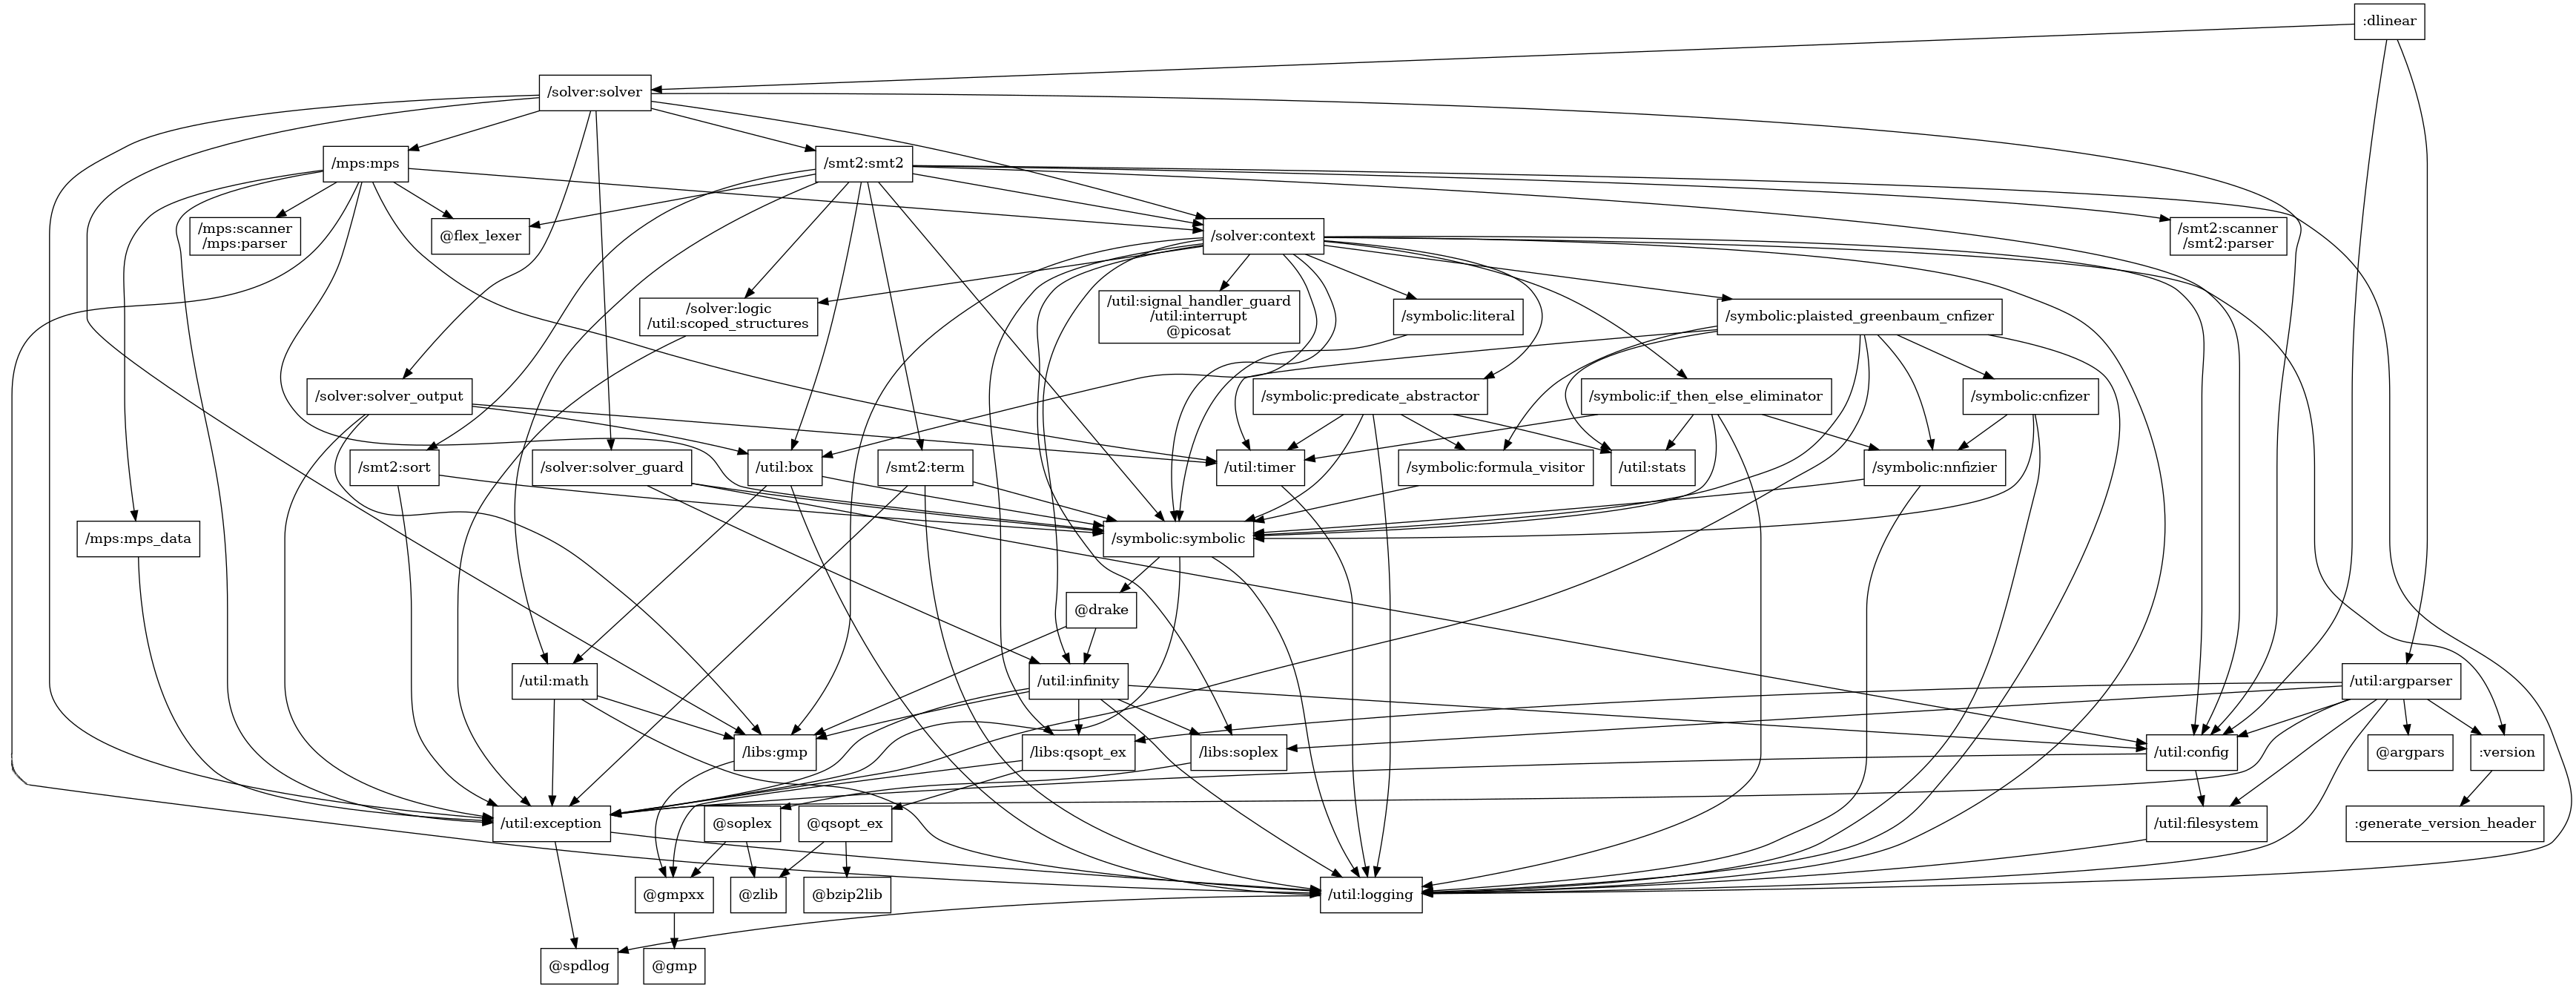
\includegraphics[width=\textwidth]{dlinear_deps}
    \caption{Visualization of the dependency graph of \dlinear as seen by \bazel}\label{fig:dlinear-deps}
\end{figure}
